\documentclass[10pt]{beamer}
\usepackage{hyperref}
\usepackage[utf8x]{inputenc}
\usepackage{graphicx}
\usepackage[nodayofweek]{datetime}
\usepackage[colorinlistoftodos]{todonotes}
\usepackage{graphicx}
\usepackage{mathtools}
\usepackage{amssymb}
\usepackage{amsmath}
\usepackage{bbm}
\usepackage{pdflscape}
\usepackage{caption}
\usepackage{subcaption}
\usepackage[T1]{fontenc}
\usepackage{authblk}
\usepackage{pdfpages}
\usepackage{setspace} 
\usepackage{booktabs}
\usepackage{longtable}
\usepackage{float}
\usepackage{tikz}
\usepackage{bm}
\usepackage{appendixnumberbeamer}
\usepackage{siunitx}
% \usepackage{natbib}
\usepackage[style=authoryear,backend=biber]{biblatex}
\usepackage{bibentry}

% \nobibliography*
\addbibresource{library.bib}

% ------------------------------------------------------------------------------
% Use the beautiful metropolis beamer template
% ------------------------------------------------------------------------------
\usepackage[T1]{fontenc}
\usepackage{fontawesome}
\usepackage{FiraSans} 
\usepackage{fontspec}
\setmonofont{Fira Mono}
\mode<presentation>
{
  \usetheme[progressbar=foot,numbering=fraction,background=light]{metropolis} 
  \usecolortheme{default} % or try albatross, beaver, crane, ...
  \usefonttheme{default}  % or try serif, structurebold, ...
  \setbeamertemplate{navigation symbols}{}%[appendixframenumber]
  % \setbeamertemplate{caption}[numbered]
  %\setbeamertemplate{frame footer}{My custom footer}
} 

\setbeamertemplate{section in toc}{\hspace*{1em}\inserttocsectionnumber.~\inserttocsection\par}
\setbeamertemplate{subsection in toc}{\hspace*{2em}\inserttocsectionnumber.\inserttocsubsectionnumber.~\inserttocsubsection\par}

\setbeamertemplate{footnote}{%
  \parindent 1em\noindent%
  \raggedright
  \tiny\insertfootnotetext\par%
}

\makeatletter
\addtobeamertemplate{footline}{%
  \vskip1ex%
  {\usebeamerfont{footnote}%
   \usebeamercolor[fg]{footnote}%
   \insertfootnotetext\par}%
}{}
\makeatother

% ------------------------------------------------------------------------------
% beamer doesn't have texttt defined, but I usually want it anyway
% ------------------------------------------------------------------------------
\let\textttorig\texttt
\renewcommand<>{\texttt}[1]{%
  \only#2{\textttorig{#1}}%
}

% ------------------------------------------------------------------------------
% minted
% ------------------------------------------------------------------------------
\usepackage{minted}


% ------------------------------------------------------------------------------
% tcolorbox / tcblisting
% ------------------------------------------------------------------------------
\usepackage{xcolor}
\definecolor{codecolor}{HTML}{FFC300}

\usepackage{tcolorbox}
\tcbuselibrary{most,listingsutf8,minted}

\tcbset{tcbox width=auto,left=1mm,top=1mm,bottom=1mm,
right=1mm,boxsep=1mm,middle=1pt}

\newtcblisting{myr}[1]{colback=codecolor!5,colframe=codecolor!80!black,listing only, 
minted options={numbers=left, style=tcblatex,fontsize=\tiny,breaklines,autogobble,linenos,numbersep=3mm},
left=5mm,enhanced,
title=#1, fonttitle=\bfseries,
listing engine=minted,minted language=r}


% ------------------------------------------------------------------------------
% Listings
% ------------------------------------------------------------------------------
\definecolor{mygreen}{HTML}{37980D}
\definecolor{myblue}{HTML}{0D089F}
\definecolor{myred}{HTML}{98290D}

\usepackage{listings}

% the following is optional to configure custom highlighting
\lstdefinelanguage{XML}
{
  morestring=[b]",
  morecomment=[s]{<!--}{-->},
  morestring=[s]{>}{<},
  morekeywords={ref,xmlns,version,type,canonicalRef,metr,real,target}% list your attributes here
}

\lstdefinestyle{myxml}{
language=XML,
showspaces=false,
showtabs=false,
basicstyle=\ttfamily,
columns=fullflexible,
breaklines=true,
showstringspaces=false,
breakatwhitespace=true,
escapeinside={(*@}{@*)},
basicstyle=\color{mygreen}\ttfamily,%\footnotesize,
stringstyle=\color{myred},
commentstyle=\color{myblue}\upshape,
keywordstyle=\color{myblue}\bfseries,
}

% Need valign for slide with equation and image
\usepackage{adjustbox}

% ------------------------------------------------------------------------------
% The Document
% ------------------------------------------------------------------------------

\begin{document}

\title{A clustering framework for conditional extremes models}

\newdate{date}{14}{05}{2025}
\date{
  \footnotesize Conference on Applied Statistics in Ireland (CASI) Talk, \\
  \displaydate{date}, \\
  \emph{Paddy O'Toole, University of Bath} \\
  \emph{Supervised by Christian Rohrbeck and Jordan Richards (University of Edinburgh)}
}

\begin{frame}[noframenumbering, plain]
  \titlepage
\end{frame}

% \begin{frame}
%   \addtocounter{framenumber}{-1}
%   % \item Get down to 20ish slides before Christian meeting
%   % \item Cut down on words wherever possible
%   % \item Do TODOs
%   \item Add QR code slide
%   % \item Fix clipping plots (requires saving manually!) (including appendix!)
%   % \item Check slide titles, don't capitalise
%   % \item Swap pdfs for pngs
%   % \item Finalise plots
%   % \item Add appendix slides + plots
%   % \item Remove commented slides when finished
%   \item Write script
%   % Full presentation notes
%   % \item Remove references to GPD
%   % \item Update simulation slides/plots (or don't)
%   % \item Go through Christians notes on slides
%   % \item Cut down on words
%   % \item Update chi plot
%   % \item Remove medians from clustering map
%   % \item Add diagnostic plots
%   % \item Comment (and do) todos (temporarily)
% \end{frame}

%=================================================

% \begin{frame}
% \frametitle{Table of contents}
% \tableofcontents
% \end{frame}

\section{Introduction}


% Images of Pulteney Bridge Weir and plaque
% Frank Greenhalgh, Engineer who designed Pulteney Weir and Sluce for Bristol Avon River Authority
\begin{frame}
   \begin{minipage}{0.5\textwidth}
     \begin{center}
       \hspace*{-0.7cm} 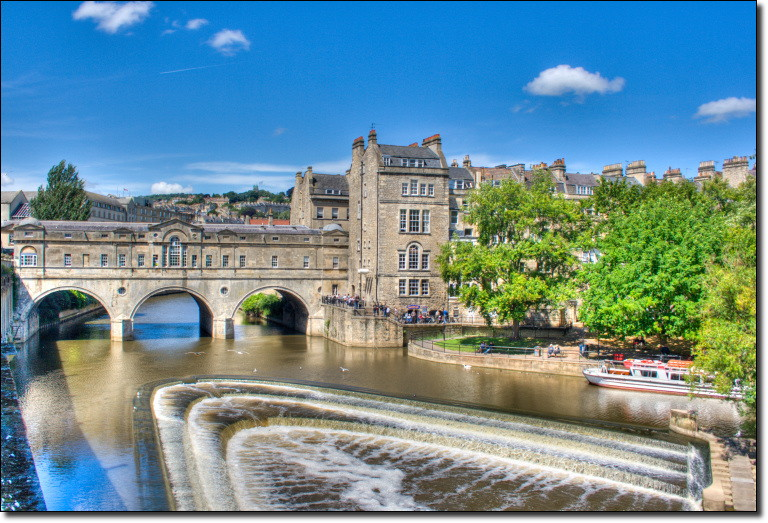
\includegraphics[width=1.4\textwidth]{images/pultney-bridge.jpg}
     \end{center}
   \end{minipage}
   \hfill
   \begin{minipage}{0.4\textwidth}
     \hspace*{0.8cm} 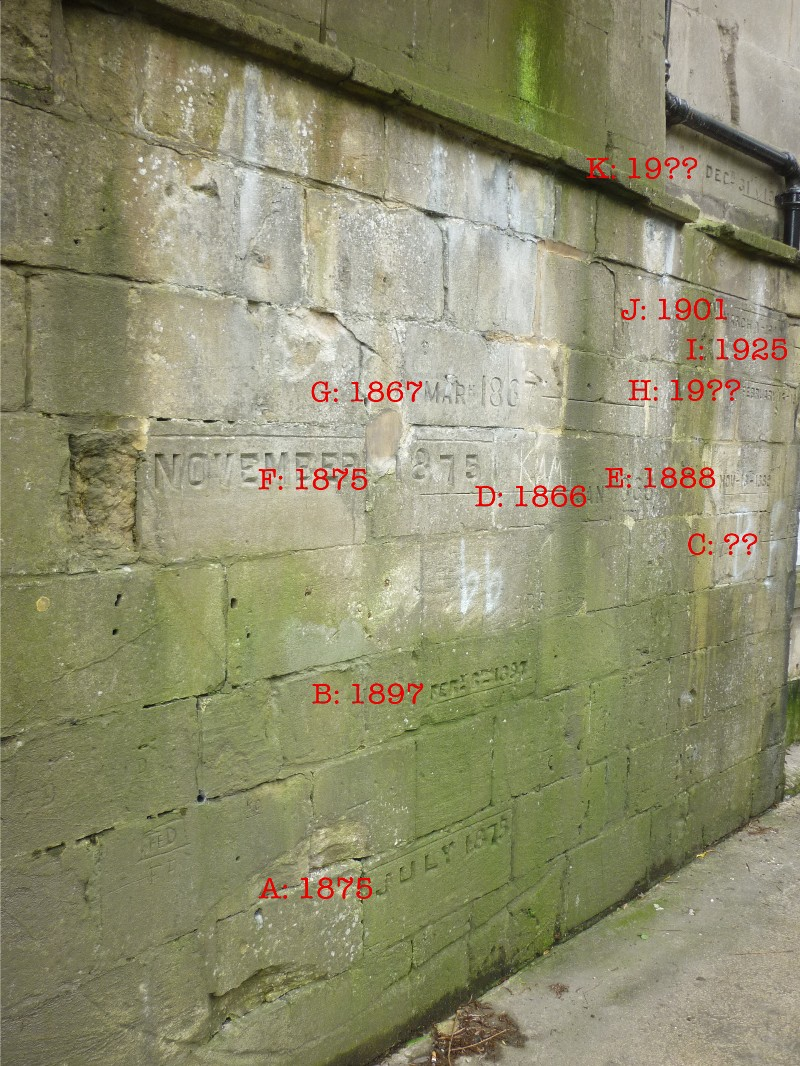
\includegraphics[width=1\textwidth]{images/Hapennybr_lower.jpg} 
   \end{minipage}
\end{frame}

\begin{frame}{Problem} 
  \begin{itemize}
    \item Often want to estimate
      \[
        \mathbb{P}(X > x, Y > y) = \textcolor{red}{\mathbb{P}(Y > y \mid X > x)}\textcolor{blue}{\mathbb{P}(X > x)}
      \]
      for large $x, y$
    \item ``concomitant''/concurrent extreme events for random vector $\bf{X}$ often particularly devastating
    \item Goal: \textbf{identify trends by clustering sites with similar \textcolor{red}{tail dependence}}
  \end{itemize}
\end{frame}

\section{Dependence Modelling}

\begin{frame}[fragile]{Asymptotic dependence}
  % reserve space for your citation block
  \newlength{\TopBoxHeight}
  \setlength{\TopBoxHeight}{\dimexpr\textheight-3cm\relax}

  \vbox to \TopBoxHeight{
    \vfill
    \begin{center}
      \begin{itemize}
        \item Coefficient of extremal dependence $\chi\in[0,1]$, 
              \[
                \chi = \lim_{u\to1}\mathbb{P}\bigl[F_1(X_1)>u\mid F_2(X_2)>u\bigr]
              \]
        \item (Increasingly strong) asymptotic dependence for $\chi > 0$.
        \item However, $\chi$ only gives summary; inference requires \textbf{dependence model}.
      \end{itemize}
    \end{center}
    \vfill
  }

  \vspace{1.5cm}
  {\scriptsize
    \rule{\linewidth}{0.4pt}\\
    \makebox[\linewidth]{
      \citeauthor{Coles1999}, \emph{\citetitle{Coles1999}} (1999)
    }
  }
\end{frame}

\begin{frame}{Ireland}
  \begin{minipage}{0.4\textwidth}
      \begin{itemize}
        \item Precipitation\textsuperscript{1} \& wind speed\textsuperscript{2} data for 59 sites across Ireland, Winter months (Oct-Mar) 1990-2020
      \end{itemize}
  \end{minipage}
  \begin{minipage}{0.59\textwidth}
    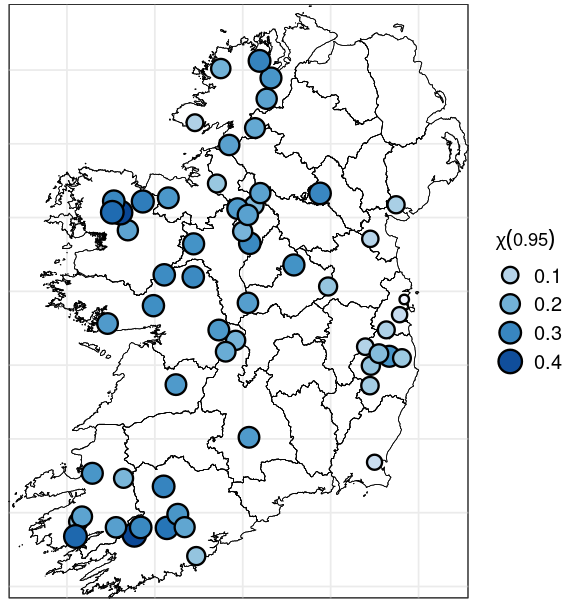
\includegraphics[width = \linewidth]{plots/041_chi_plots_man_crop.png}
  \end{minipage}
  {\scriptsize
    \rule{\linewidth}{0.4pt}\\
    \makebox[\linewidth]{
      \textsuperscript{1} Met Éireann weekly aggregate
      \hfill{}
      \textsuperscript{2} ERA5 reanalysis weekly mean of daily maxima
      \hspace{0.5cm}
    }
  }
\end{frame}

\section{Conditional extremes}

\begin{frame}{Marginal transformation}
  % allows for heteroskedastic regression model, symmetry means model is the same
  % for both positive and negative dependence, and also easy to model any
  % dependence strength
  \center
  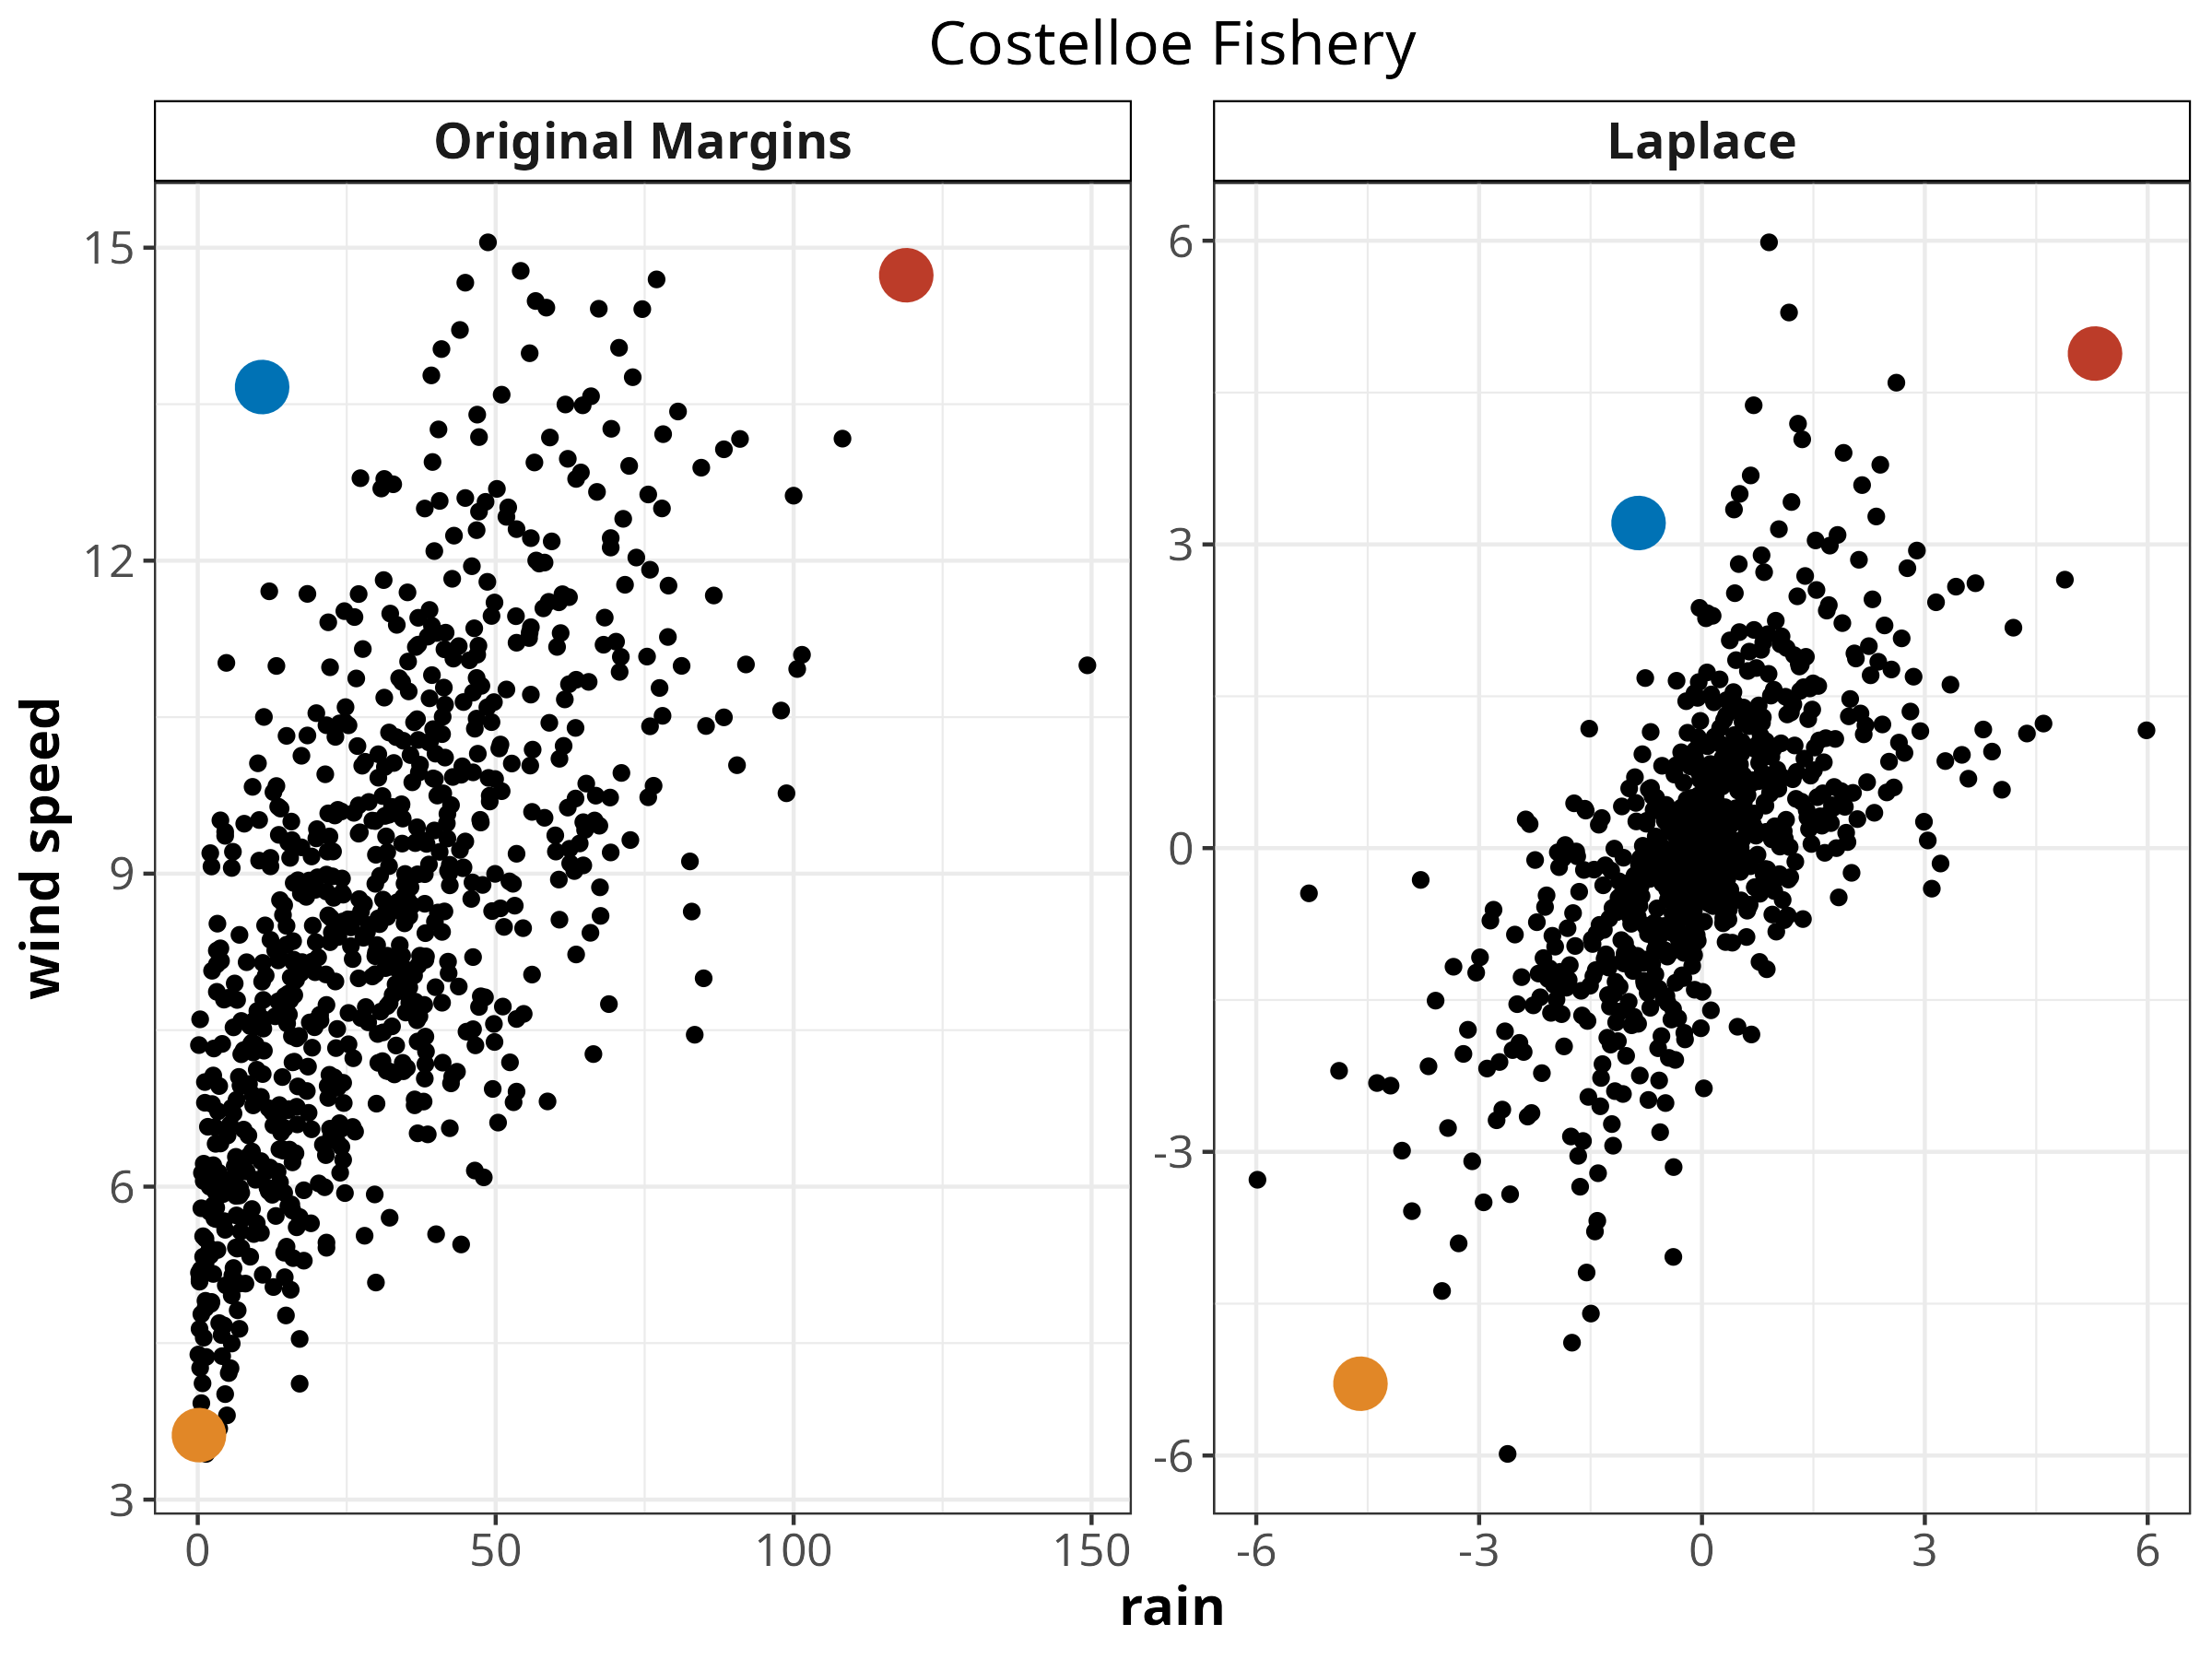
\includegraphics[width=0.9\textwidth]{plots/transform_costelloe.png} 
  % {\scriptsize
  %   \rule{\linewidth}{0.4pt}\\
  %   \makebox[\linewidth]{
  %     \citeauthor{Keef2013}, \emph{\citetitle{Keef2013}} (2013)
  %   }
  % }
\end{frame}

% Multivariate piecewise function, Z, Y independent
\begin{frame}[t]{Conditional extremes}
% Reduces multivariate model to simple univariate models!
\begin{itemize}
  \item \textbf{Heteroskedastic regression dependence model}: 
  \begin{equation*}
      % \bm{Y}_{-i} \mid Y_i = y_i = \bm{\alpha}_{\mid i}\bm{y}_i + \bm{y}_i^{\bm{\beta}_{\mid i}}\bm{Z}_{\mid i}, y_i > u_{Y_i},
    Y \mid X = x = \alpha x + x^{\beta} Z, \text{ for } x > u
  \end{equation*}
  \vspace{-5mm}
  % with
  \begin{itemize}
    \item slope parameter $\alpha$  for $Y$ given large $X$,
    \item ``spread'' parameter $\beta \in (-\infty, 1]$ controls stochasticity of relationship between $Y$ and large $X$. 
  \end{itemize}
\end{itemize}
\end{frame}

\begin{frame}[t]{Conditional extremes}
% Reduces multivariate model to simple univariate models!
\begin{itemize}
  \item <1-> \textbf{Heteroskedastic regression dependence model}: 
  \begin{equation*}
      \bm{Y}_{-i} \mid Y_i = y_i = \bm{\alpha}_{\mid i}\bm{y}_i + \bm{y}_i^{\bm{\beta}_{\mid i}}\bm{Z}_{\mid i}, \text{ for } y_i > u_{Y_i}
  \end{equation*}
  \vspace{-5mm}
  % with
  \begin{itemize}
    \item <1-> slope parameter $\alpha_{j \mid i} \in [-1, 1]$  for $Y_j$ given large $Y_i$,
    \item <1-> ``spread'' parameter $\beta_{j \mid i} \in (-\infty, 1]$ $\bm{\beta}_{\mid i}$ controls stochasticity of relationship between $Y_j$ and large $Y_i$. 
  \end{itemize}
  \vspace{2mm}
  \item <2-> Key assumptions:
  \begin{itemize}
    \item <2-> Residuals $\bm{Z}_{\mid i} \sim N(\bm{\mu}_{\mid i}, \bm{\sigma}_{\mid i})$ 
    \item <2-> $\bm{Z}_{\mid i}, Y_i$ conditionally independent for large $Y_i$
  \end{itemize}
  \vspace{2mm}
  \item <2-> Special cases:
  \vspace{-4mm}
  \begin{alignat*}{2}
  &\bm{\alpha}_{\mid i} = 0, \bm{\beta}_{\mid i} = 0    &&\implies \bm{Y}_{-i}, \bm{Y}_{i} \text{ independent,} \\
  &\bm{\alpha}_{\mid i} = -1/1, \bm{\beta}_{\mid i} = 0 &&\implies \text{ perfect positive/negative dependence,} \\
  &-1 < \bm{\alpha}_{\mid i} < 1 && \implies \text{ asymptotic independence}
  \end{alignat*}
\end{itemize}
\vspace{-1.1cm}
{\scriptsize
  \rule{\linewidth}{0.4pt}\\
  \makebox[\linewidth]{
    \citeauthor{Heffernan2004}, \emph{\citetitle{Heffernan2004}} (2004)
  }
}
\end{frame}

\begin{frame}{Conditional extremes}
  \center{}
  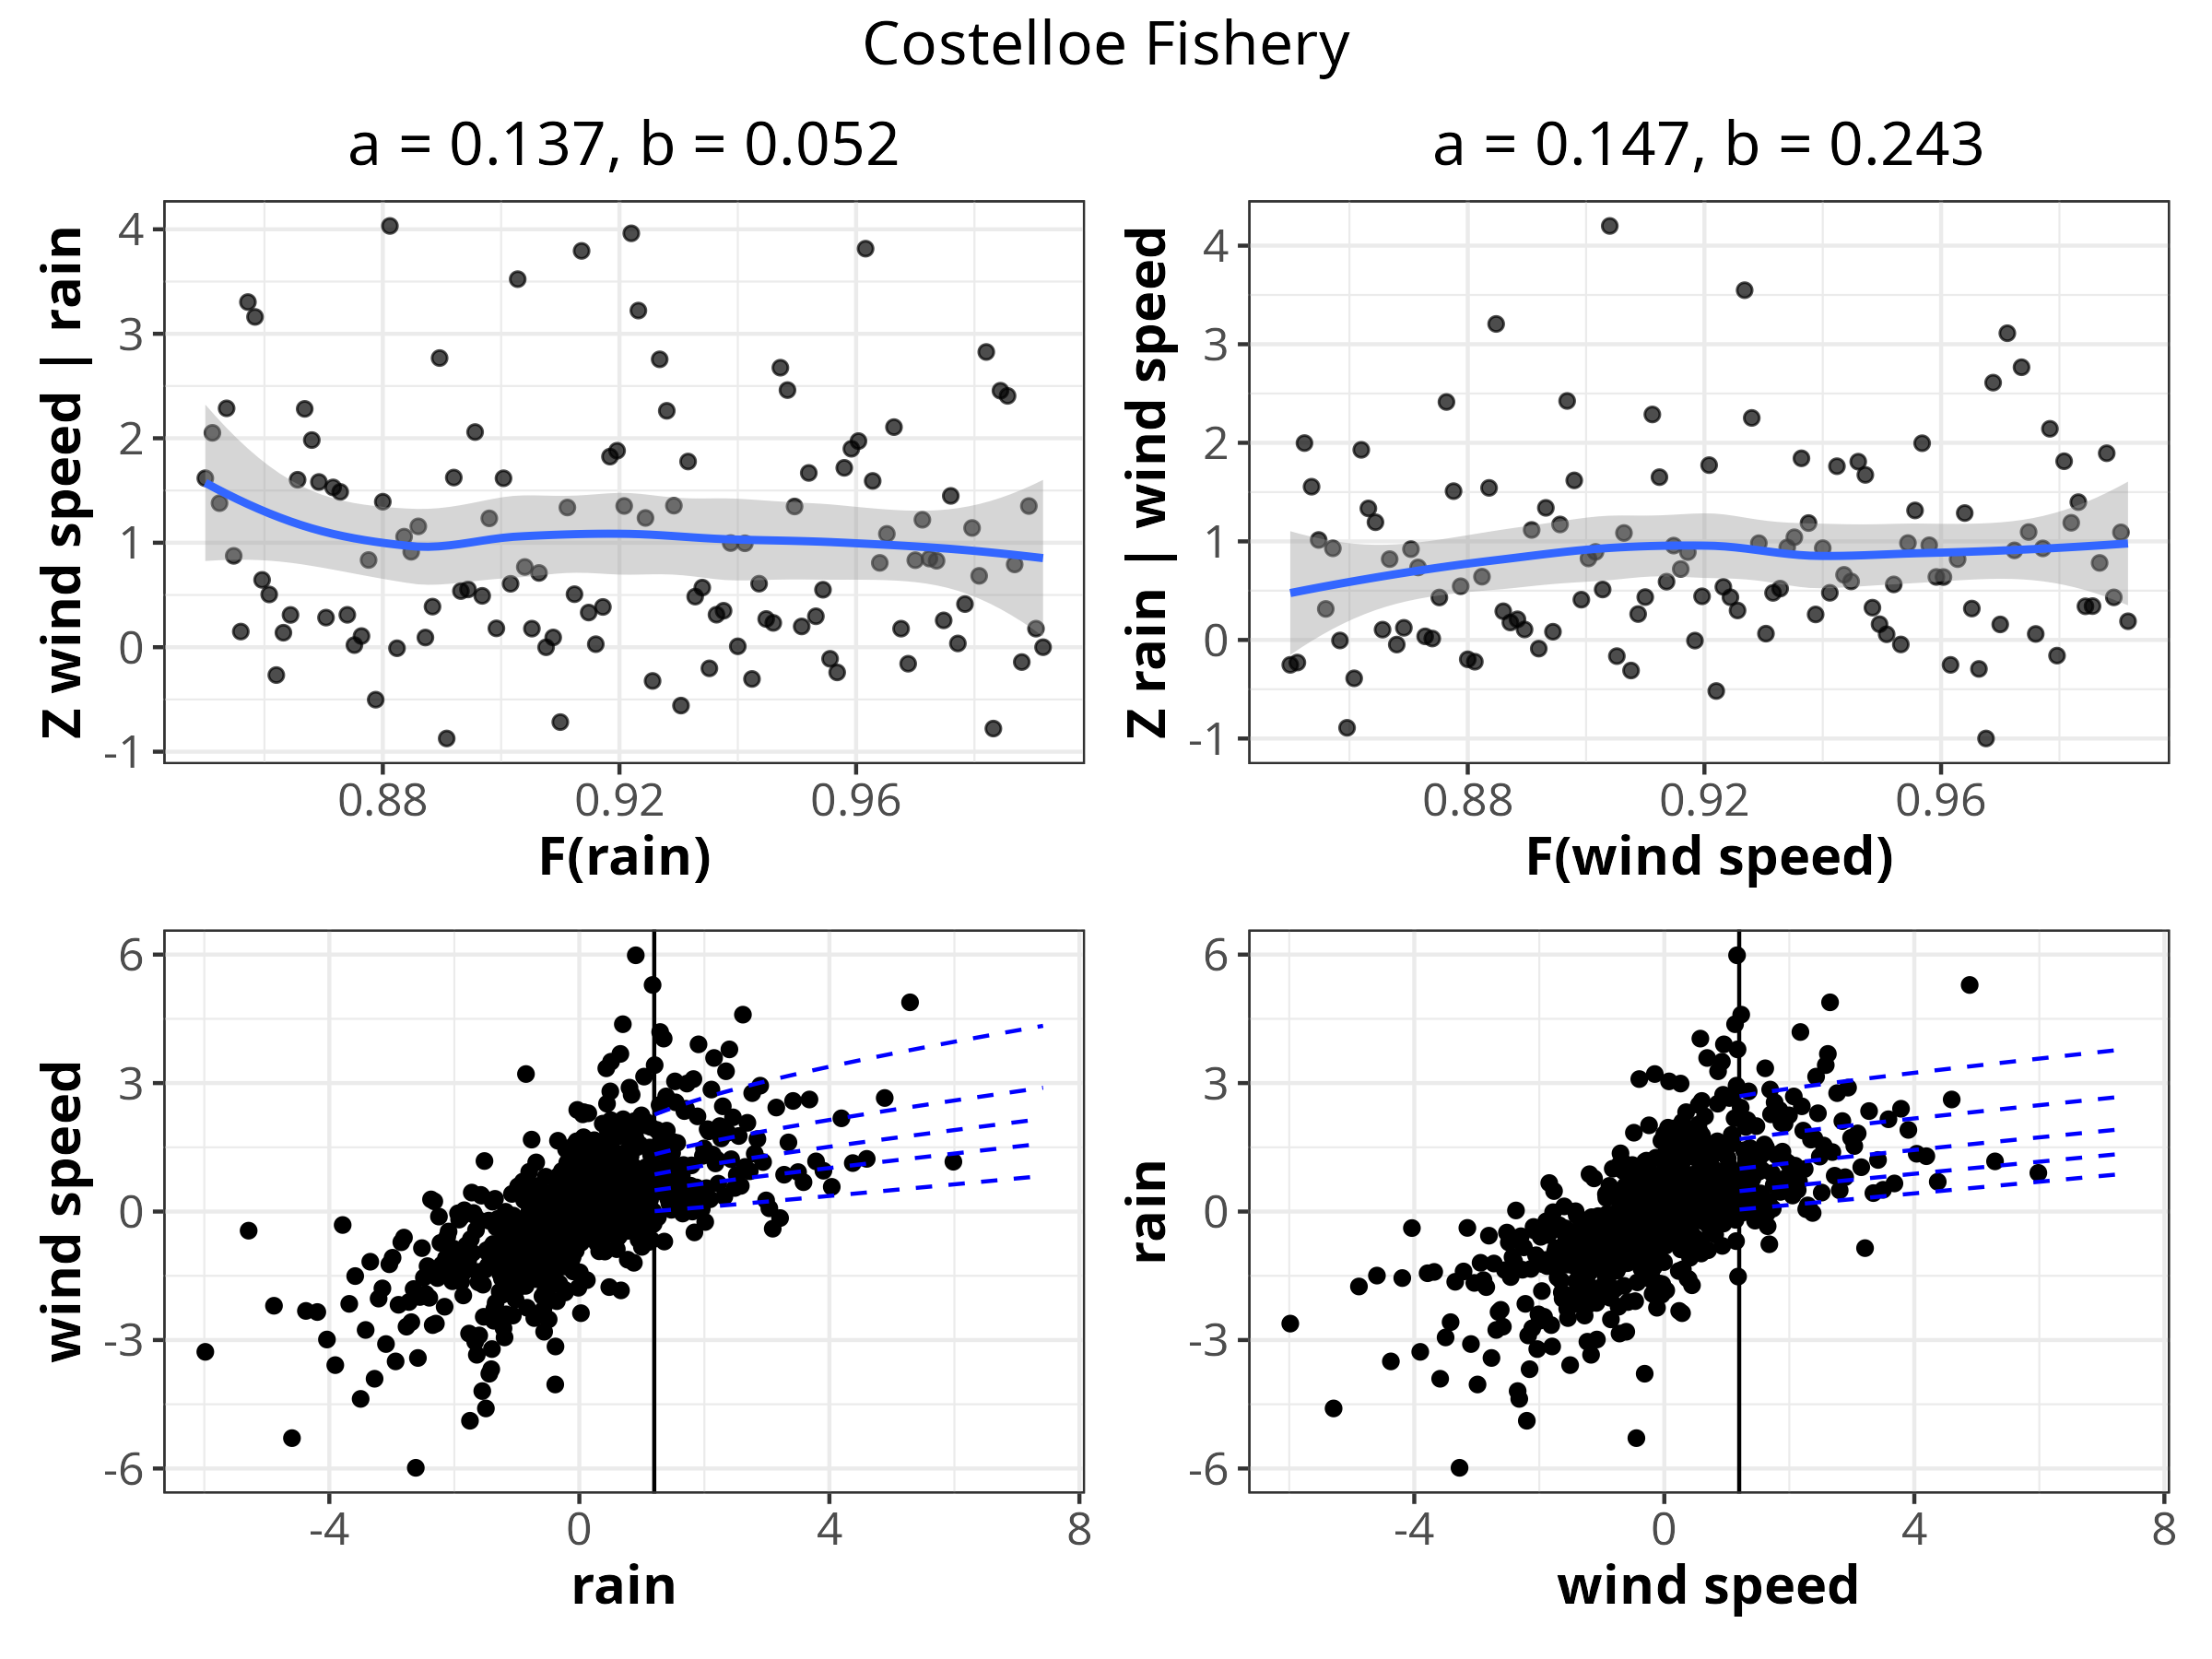
\includegraphics[width=\textwidth]{plots/041_costelloe_fishery.png} 
\end{frame}

\begin{frame}{Inference}
  \begin{itemize}
    Inference assumes conditional distribution follows diagonal multivariate Normal (MVN) distribution: \\
      \begin{equation*} \label{eq:ce_norm}
        \bm{Y}_{-i} \mid Y_i = y_i \sim N\left(\bm{\alpha}_{\mid i} y_i + y_i^{\bm{\beta}_i} \bm{\mu}_{\mid i}, y_i^{\bm{\beta}_i} \bm{\sigma_{\mid i}}\right), \text{ for } Y_i > u_{Y_i}
      \end{equation*} \\
    $\implies$ \textbf{dependence structures at different sites can be compared using their MVN distributions}
\end{itemize}
\end{frame}

\section{Clustering}

\begin{frame}{skew-geometric Jensen-Shannon divergence}
  \begin{itemize}
    \item <1-> Kullback-Leibler divergence $KL(P \mid\mid Q)$ measures (asymmetric) distance from $P$ to $Q$
    % triangle inequality: “direct” distance between two distributions is never larger than going through a third.
    \item <1-> $KL(P \mid \mid Q)$ has closed form for two MVNs
    \item <2-> Weighted geometric mean $G_{\alpha}(P, Q) = P^{\alpha} Q^{1 - \alpha}, \alpha \in [0, 1]$
    \item <3-> weighted product $G_{\alpha}$ of two exponential family members is in \textbf{same family}.
    \item <4-> \textbf{Skew-geometric Jensen-Shannon divergence}:
      \[
        JS^{G_{\alpha}}(P \mid\mid Q) = \frac{1}{2} \left\{KL(P \mid\mid G_{\alpha}(P, Q)) + KL(Q \mid\mid G_{\alpha}(P, Q))\right\}
      \]
  \end{itemize}
  \vspace{1.5cm}
  {\only<4>{\scriptsize
    \rule{\linewidth}{0.4pt}\\
    \makebox[\linewidth]{
      \citeauthor{Nielsen2019}, \emph{\citetitle{Nielsen2019}} (2019)
    }
  }}
\end{frame}

\begin{frame}{Clustering}
  \begin{itemize}
    \item Uses \textbf{k-medoids} to cluster over $JS_{G_{\alpha}}$ dissimilarity matrix between sites
    \item \textbf{Elbow plot}: $k$ chosen using \textbf{Total Within Group Sum of Squares} between sites $x$ within clusters $C_i$ with medoids $m_i$:
     \[
       \mathrm{TWGSS}(k) = \sum_{i=1}^{k}\sum_{x \in C_i} JS^{G_{\alpha}}\bigl(x \mid \mid m_i\bigr)
     \]
  \end{itemize}
  % \vspace{0.1em}
  % \vspace{-2em}
  \begin{center}
    \vspace{-0.3cm}
    
\includegraphics[width=0.6\textwidth]{plots/elbow_plot.png}
  \end{center}
\end{frame}

\section{Simulations}

\begin{frame}{Gaussian copula}
  \todo{Stop plot clipping}
  \begin{itemize}
    \item For single ``site'', generate data from bivariate Gaussian copula with correlation $\rho_{\text{Gauss}}$.
    \item (asymptotic) CE parameters are $\alpha = \rho_{\text{Gauss}}^2, \beta = 1/2$
    \item Example: 12 ``sites'' with \num[group-separator={,}]{10000} observations of 2 variables
    \item 3 clusters of 4 locations defined by respective $\rho_{Gauss}$ values of $0.3, 0.6, 0.9$.
  \end{itemize}
\end{frame}

\begin{frame}{Gaussian copula}
  \center
  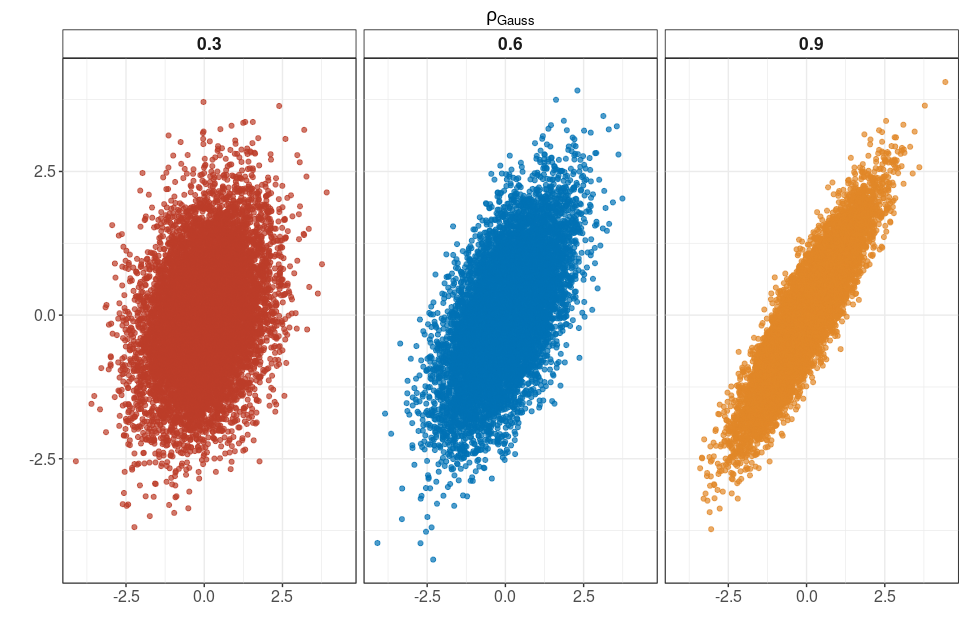
\includegraphics[width=\textwidth]{plots/gauss_sim_ex_man.png}
\end{frame}

\begin{frame}{Gaussian copula - results}
  \center
  
\includegraphics[width=\textwidth]{plots/sim_01_gauss_cop_man.png}
\end{frame}

\begin{frame}{Mixture simulation}
  \begin{itemize}
    \item <1-> Extend design to mixture of Gaussian and t-copulas
    \item <2-> Idea: 
    \begin{itemize} 
      \item Gaussian copula generates observations exhibiting extremal independence, 
      \item t-copula induces extremal dependence.
    \end{itemize}
    \item <3-> Design: 12 sites with \num[group-separator={,}]{10000} bivariate observations
    \item <3-> 2 clusters of 6 sites
    \item <4-> Grid search performed over $\rho_{gauss}, \rho_{t_1}, \rho_{t_2} \in [0, 1]$.
    \item <5-> Clustering compared to competing Vignotto algorithm using Adjusted Rand Index $\text{ARI} \in [0, 1]$ 
  \end{itemize}

  % {\scriptsize
  %   \rule{\linewidth}{0.4pt}\\
  %   \makebox[\linewidth]{
  %     \citeauthor{Vignotto2021}, \\
  %     % \emph{\citetitle{Vignotto2021}} (2021)
  %   }
  % }
  {\only<5>{\scriptsize
    \rule{\linewidth}{0.4pt}\\
    \begin{minipage}{\linewidth}
      \vspace{2mm}
      \citeauthor{Vignotto2021},\\
      \emph{\citetitle{Vignotto2021}} (2021)
    \end{minipage}
  }}
\end{frame}

\begin{frame}{Mixture simulation}
  \center
  
\includegraphics[width=1\textwidth]{plots/sim_01b_ce_vs_vi_dqu_0.9_man.png}
\end{frame}

\section{Ireland meteorological data}

% Maps of clustering
\begin{frame}{Ireland clustering}
  \center
  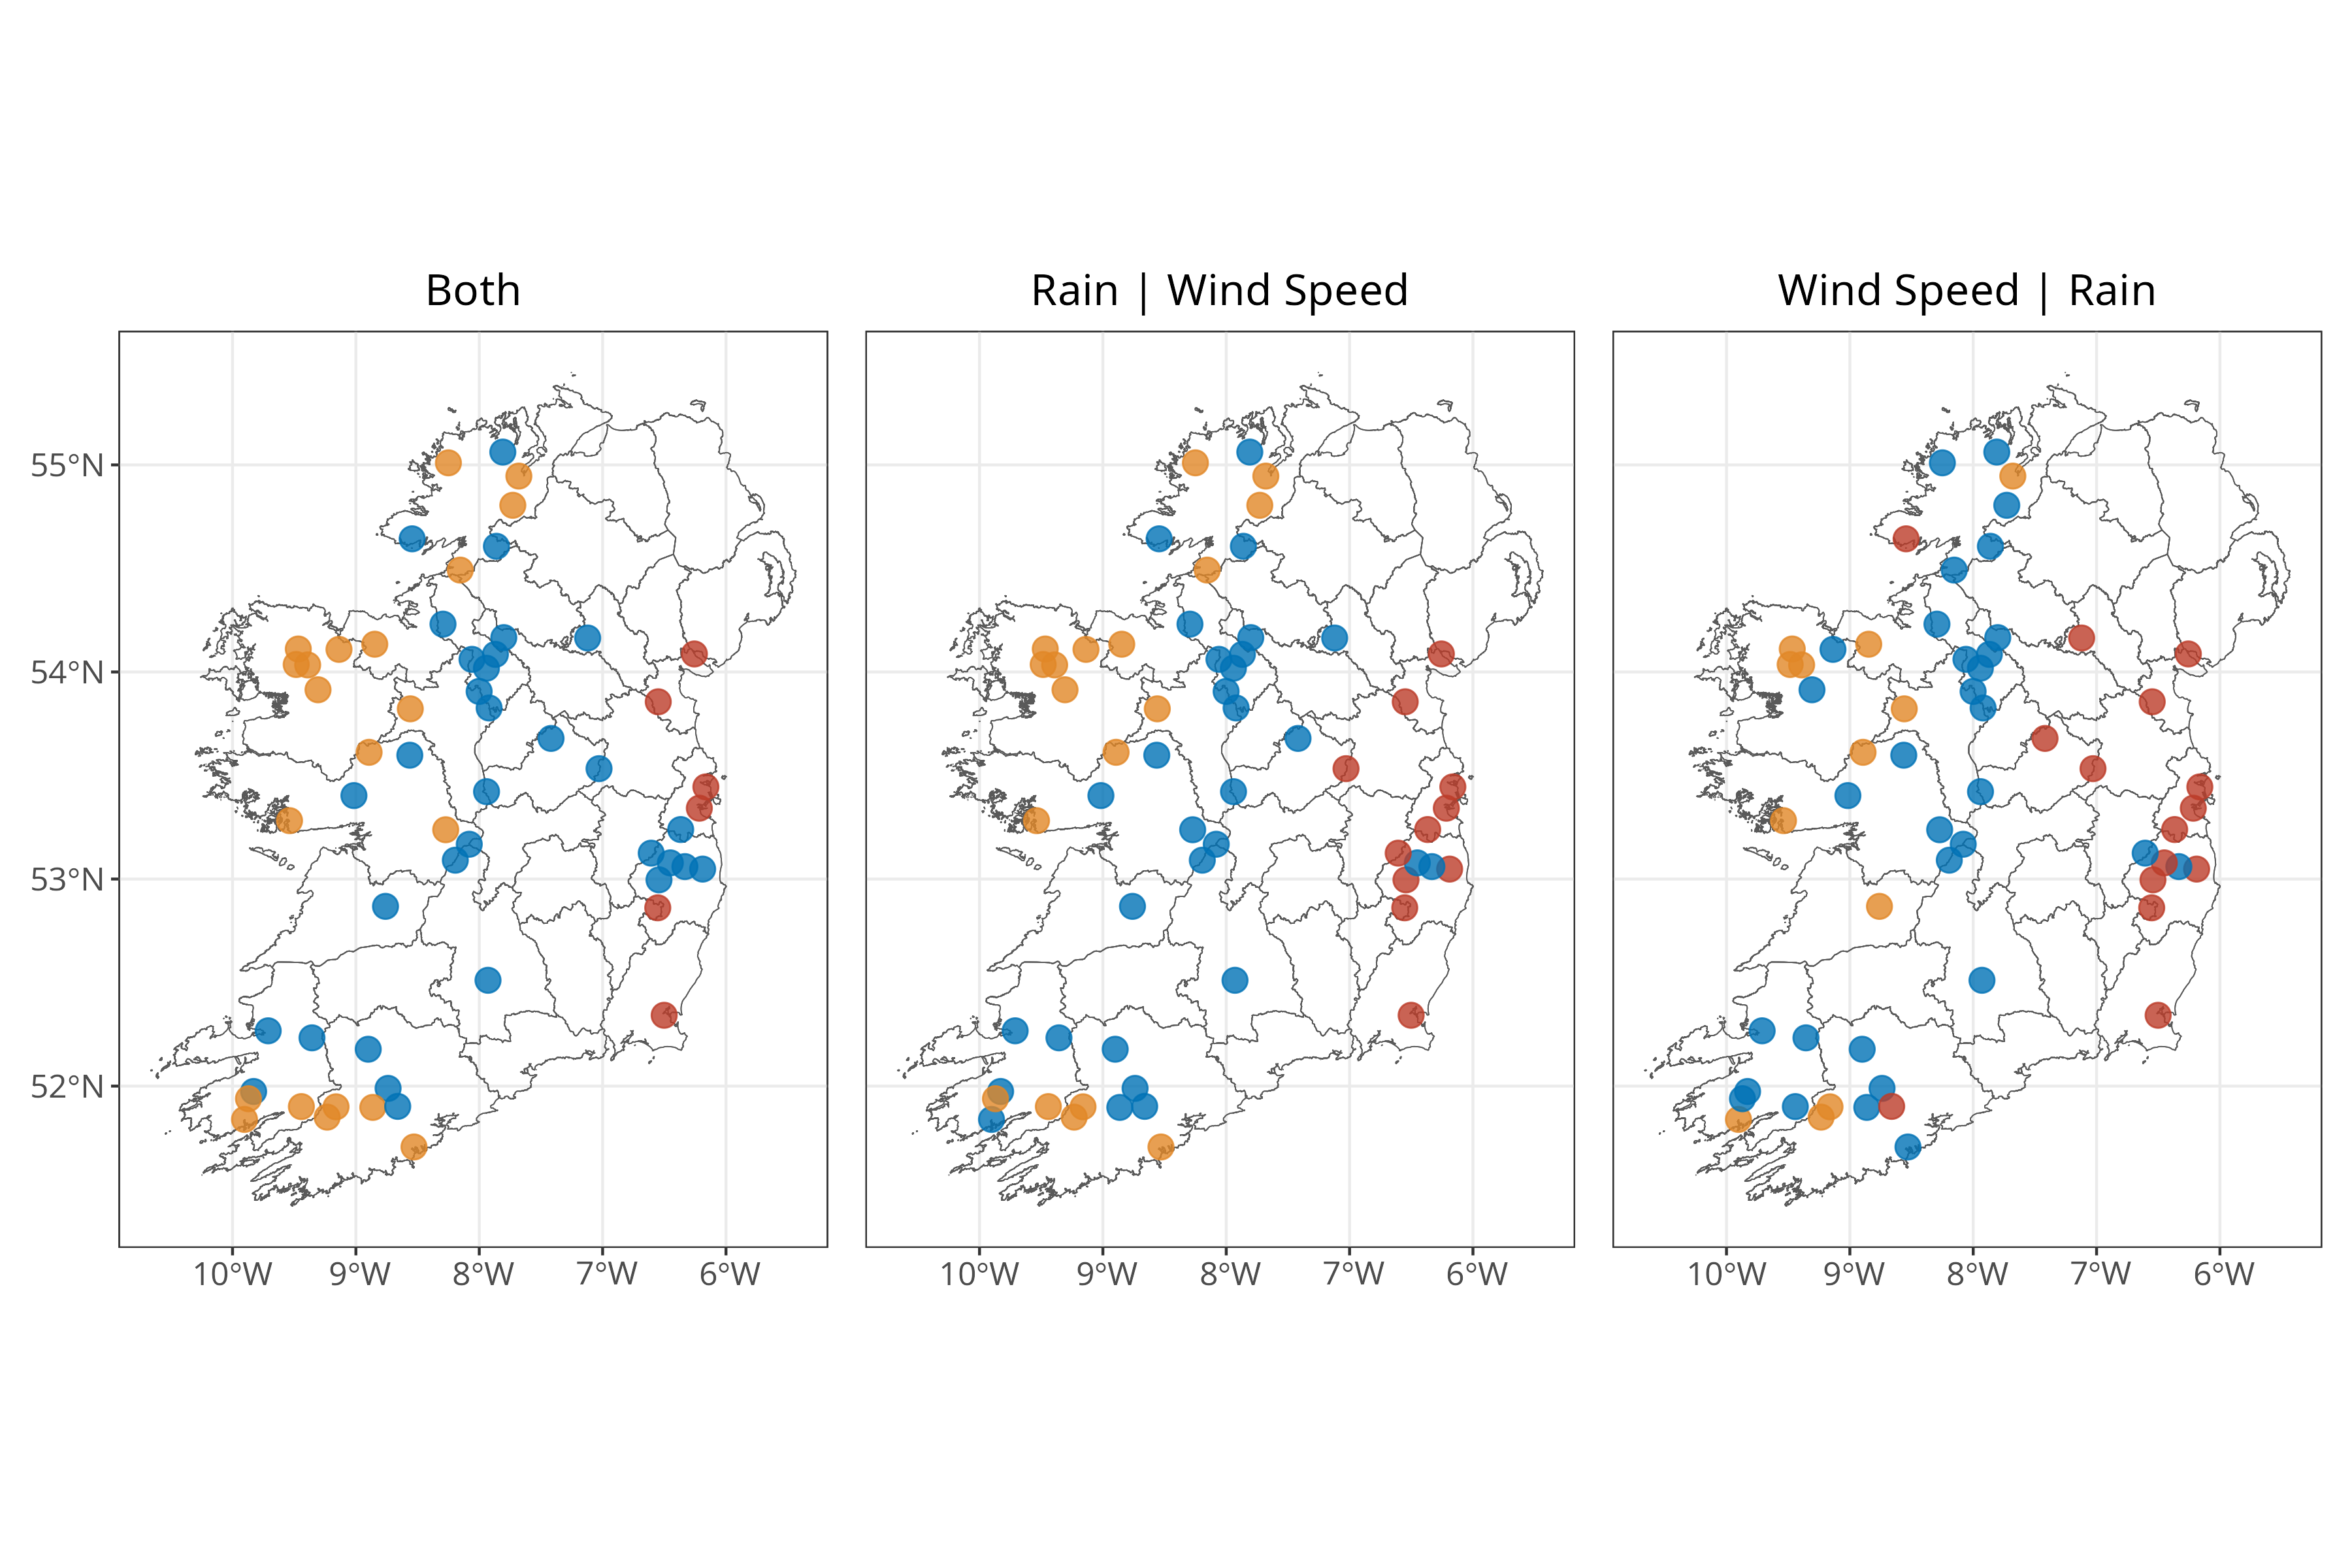
\includegraphics[width=0.9\textwidth]{plots/cluster_dqu_sep.png} 
\end{frame}

\section{Discussion}

\begin{frame}{Discussion}
  \begin{itemize}
    \item <1-> \textbf{Conclusion}:
      \begin{itemize}
        \item Principled \& effective clustering framework for CE models
        \item Simulations \& application show clustering can group sites with similar tail dependence, which may aid interpretation
      \end{itemize} 
    \vspace{2mm}
    \item <2-> \textbf{Limitations}:
      \begin{itemize}
        \item \textbf{CE}: Gaussian assumption for $\bm{Z}_{\mid i}$
        \item \textbf{Clustering}: Uncertainty in CE fits is ignored in clustering
      \end{itemize} 
  \end{itemize} 
\end{frame}

% QR Code slide
\begin{frame} 
  \addtocounter{framenumber}{-1}
  Thank you! For slides and supplementary materials, please scan the QR code below:
  \begin{center}
    
\includegraphics[width=0.5\textwidth]{images/9pW0kU.jpg}
  \end{center}
\end{frame}

\appendix

\begin{frame}\frametitle{References}
\tiny
\printbibliography[heading=none]
\end{frame}

\section{Appendix}

\begin{frame}{Mixture simulation (three variables)}
  \center
  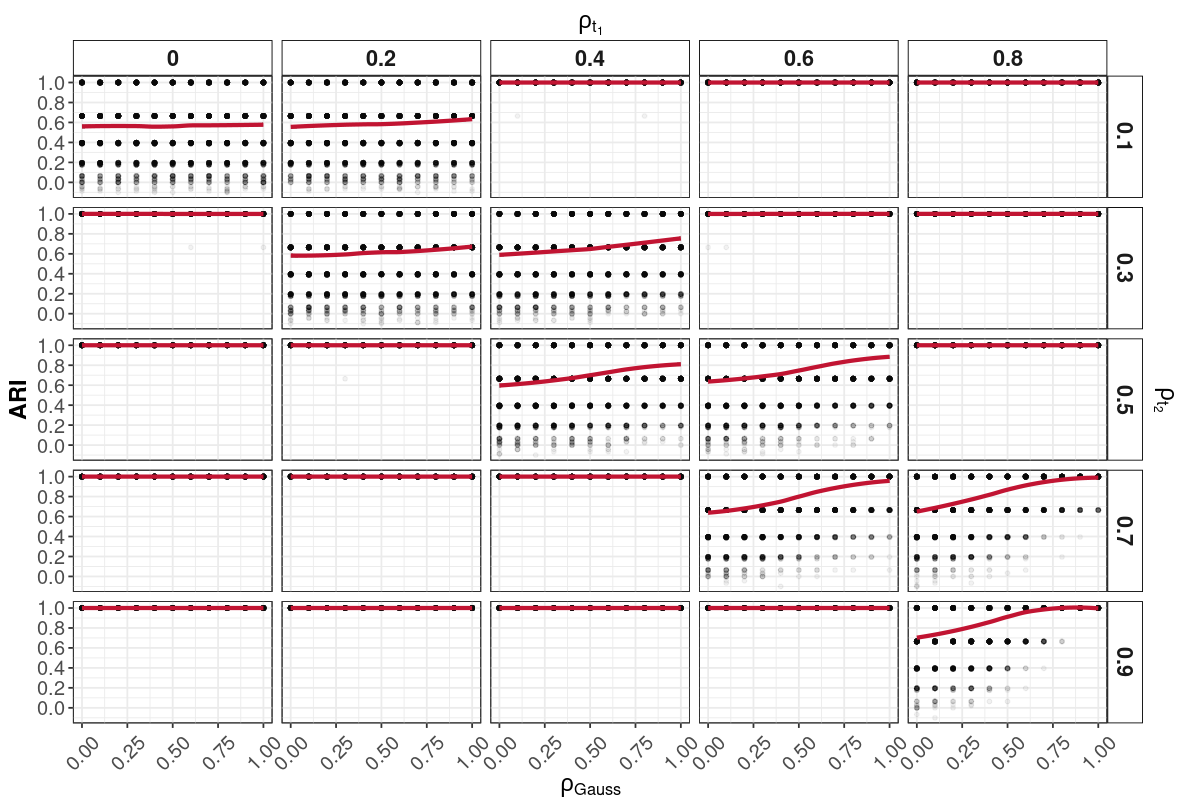
\includegraphics[width=1\textwidth]{plots/sim_01d_js_sens_3_var_dqu_0.9_man.png}
\end{frame}

\begin{frame}{More realistic example}
  \center
  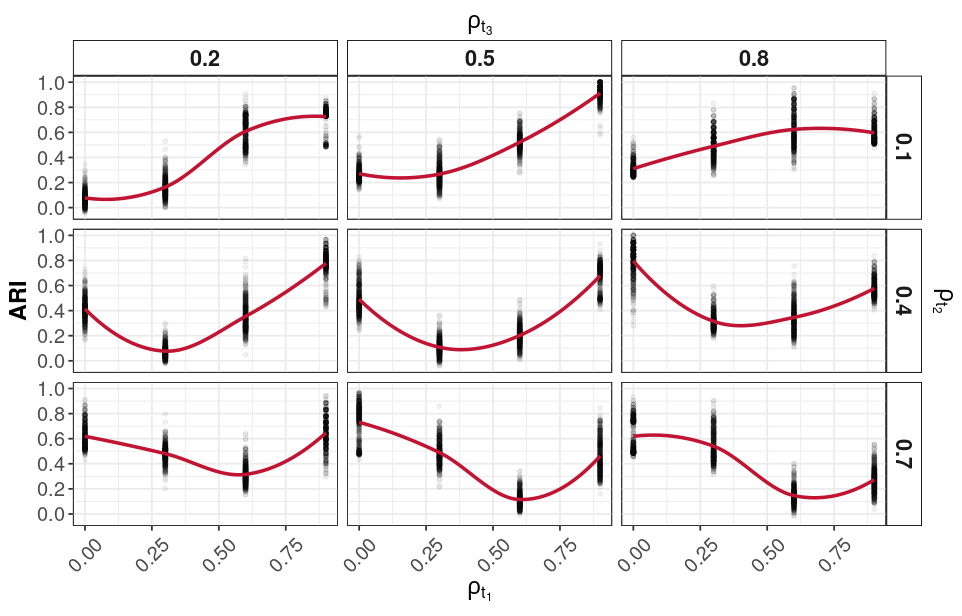
\includegraphics[width=1\textwidth]{plots/01c2_js_sens_sim_60_locs_dqu_0.9_smooth_man.png}
\end{frame}

\begin{frame}{Uncertainty Reduction}
  \center
  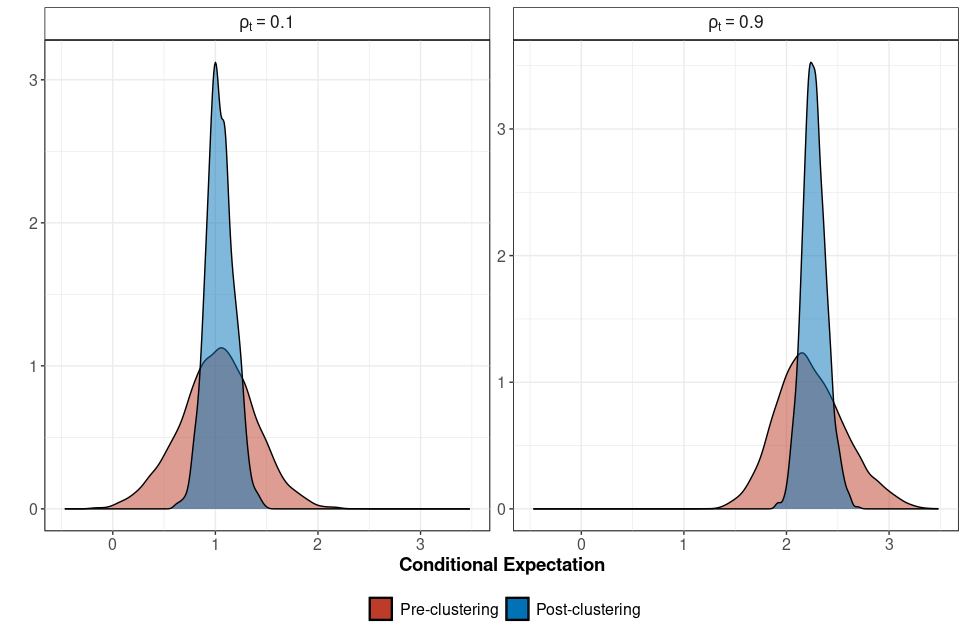
\includegraphics[width=1\textwidth]{plots/sim_01e_bootstrap_man.png}
\end{frame}

\begin{frame}{$\alpha, \beta$ pre-clustering}
  \center
  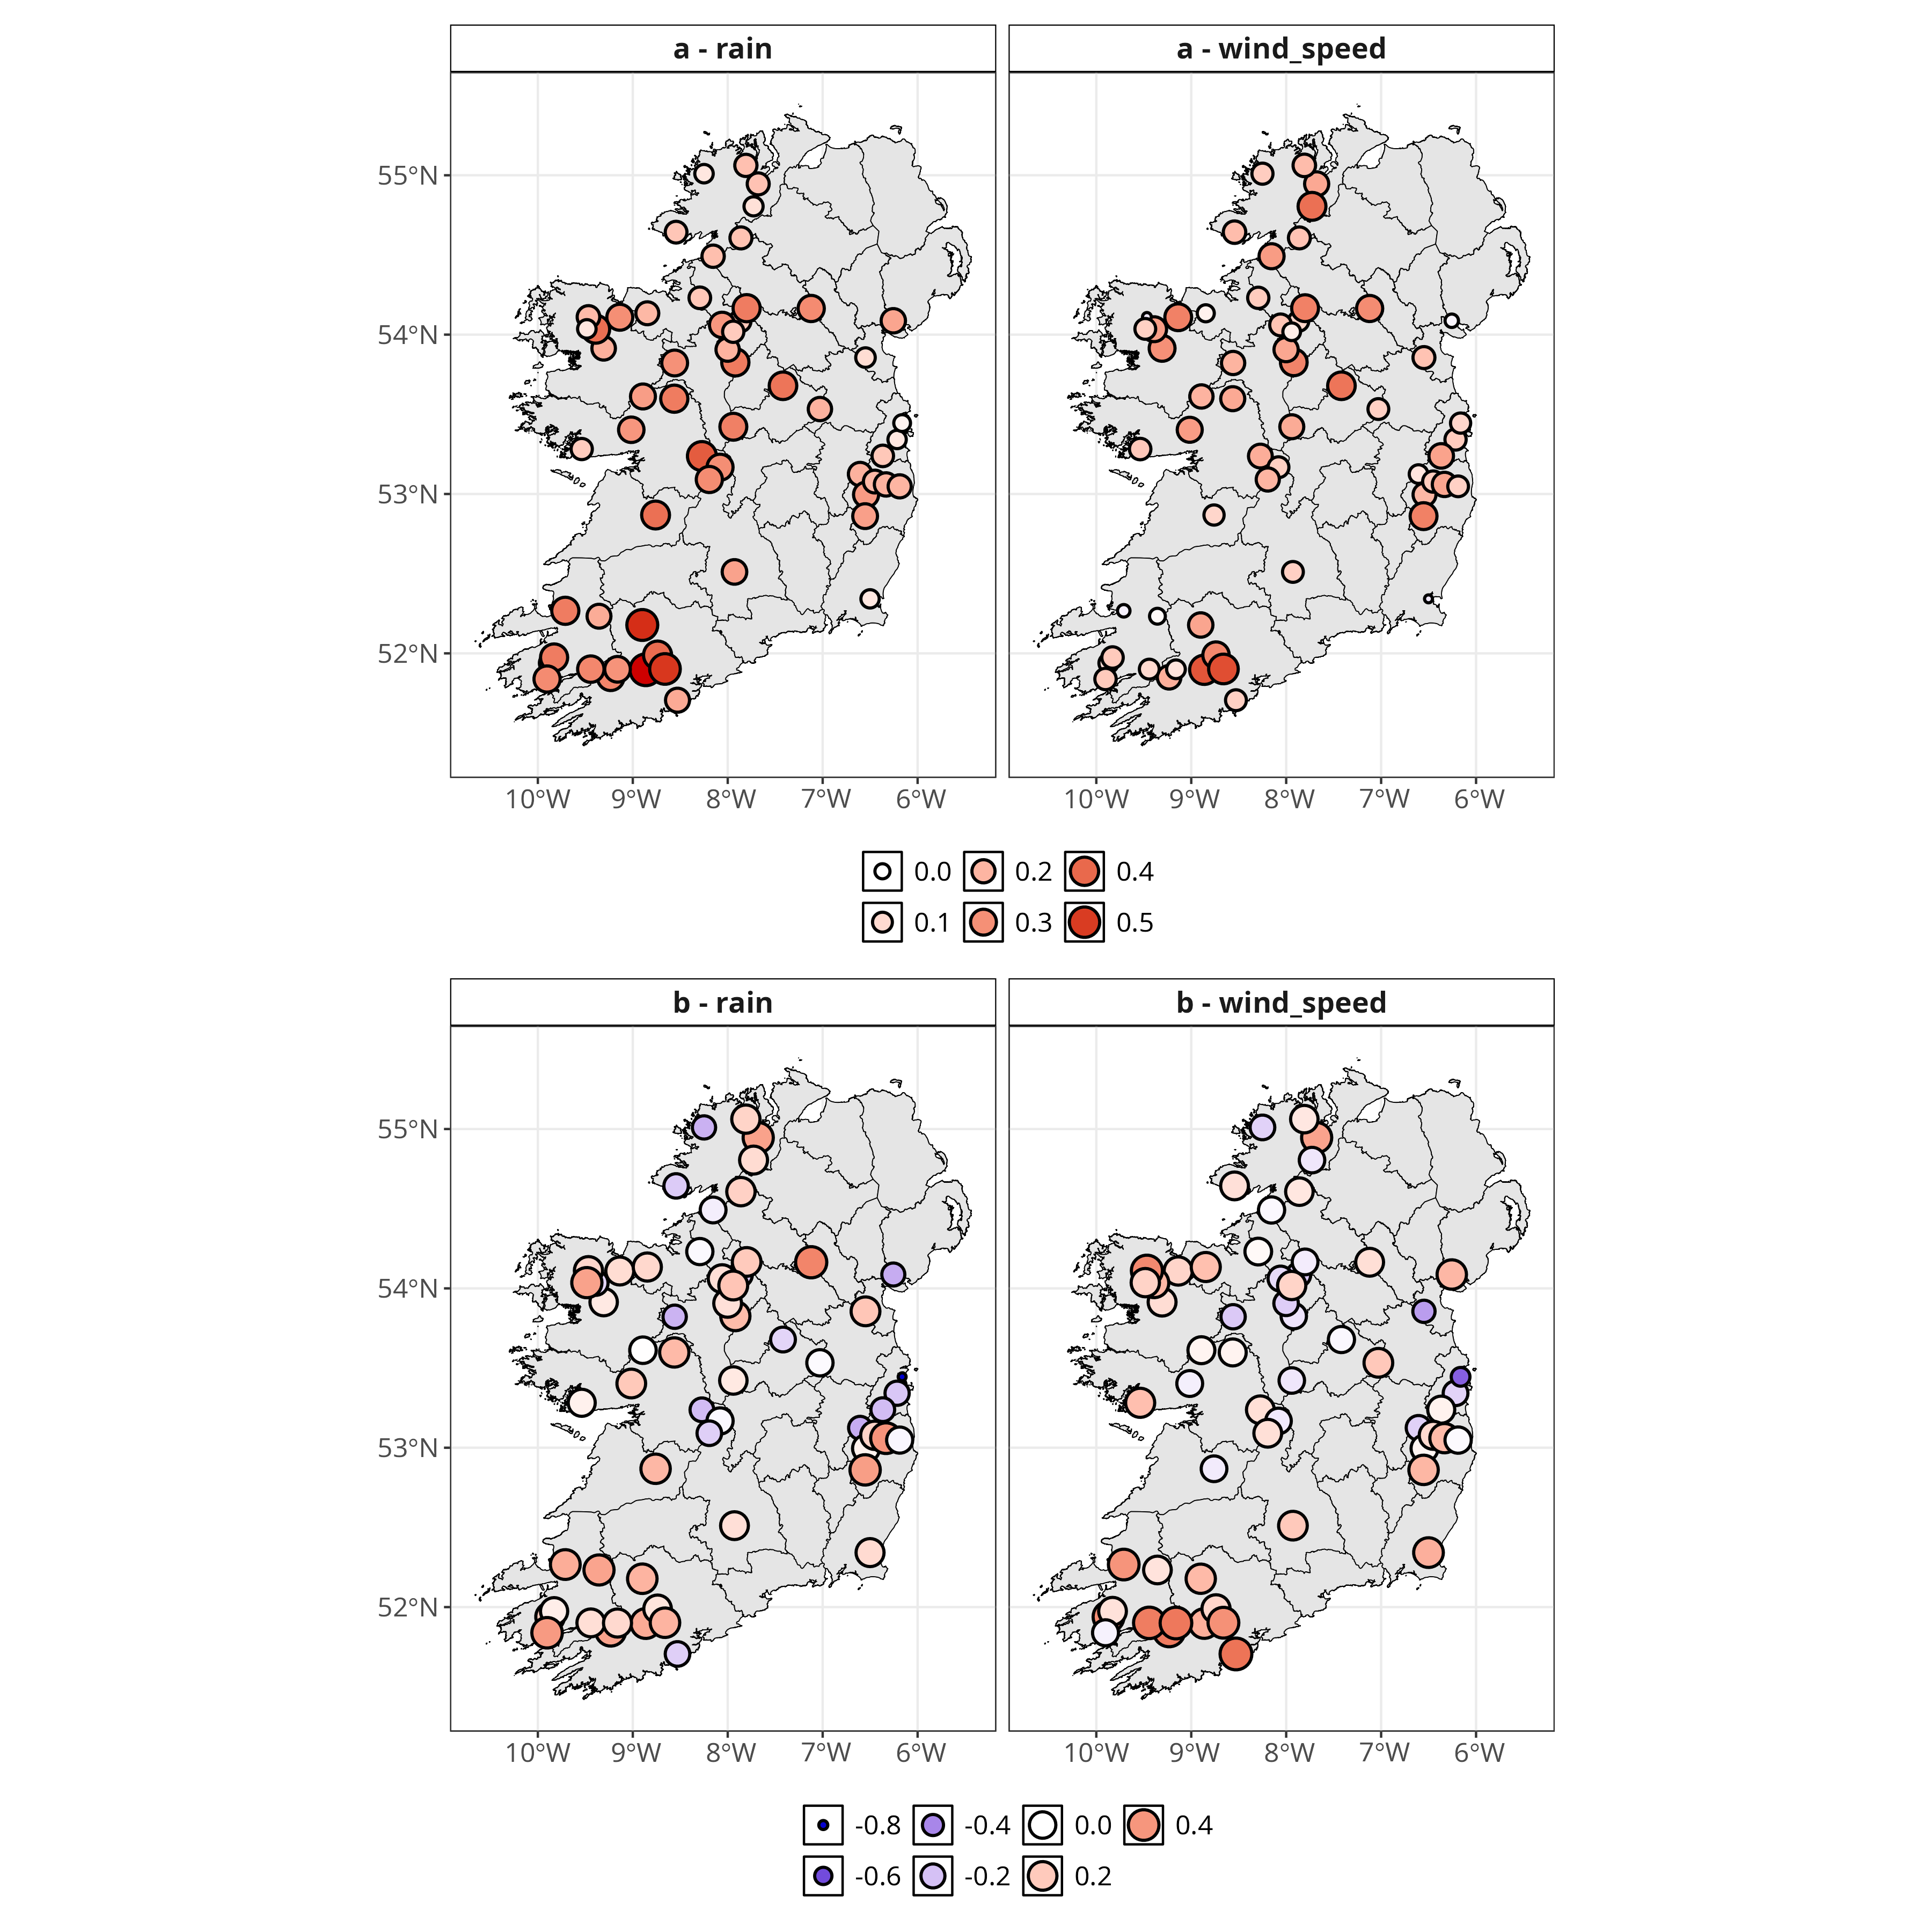
\includegraphics[width=0.75\textwidth]{plots/ire_ce.png} 
\end{frame}

\begin{frame}{$\alpha, \beta$ post-clustering}
  \center
  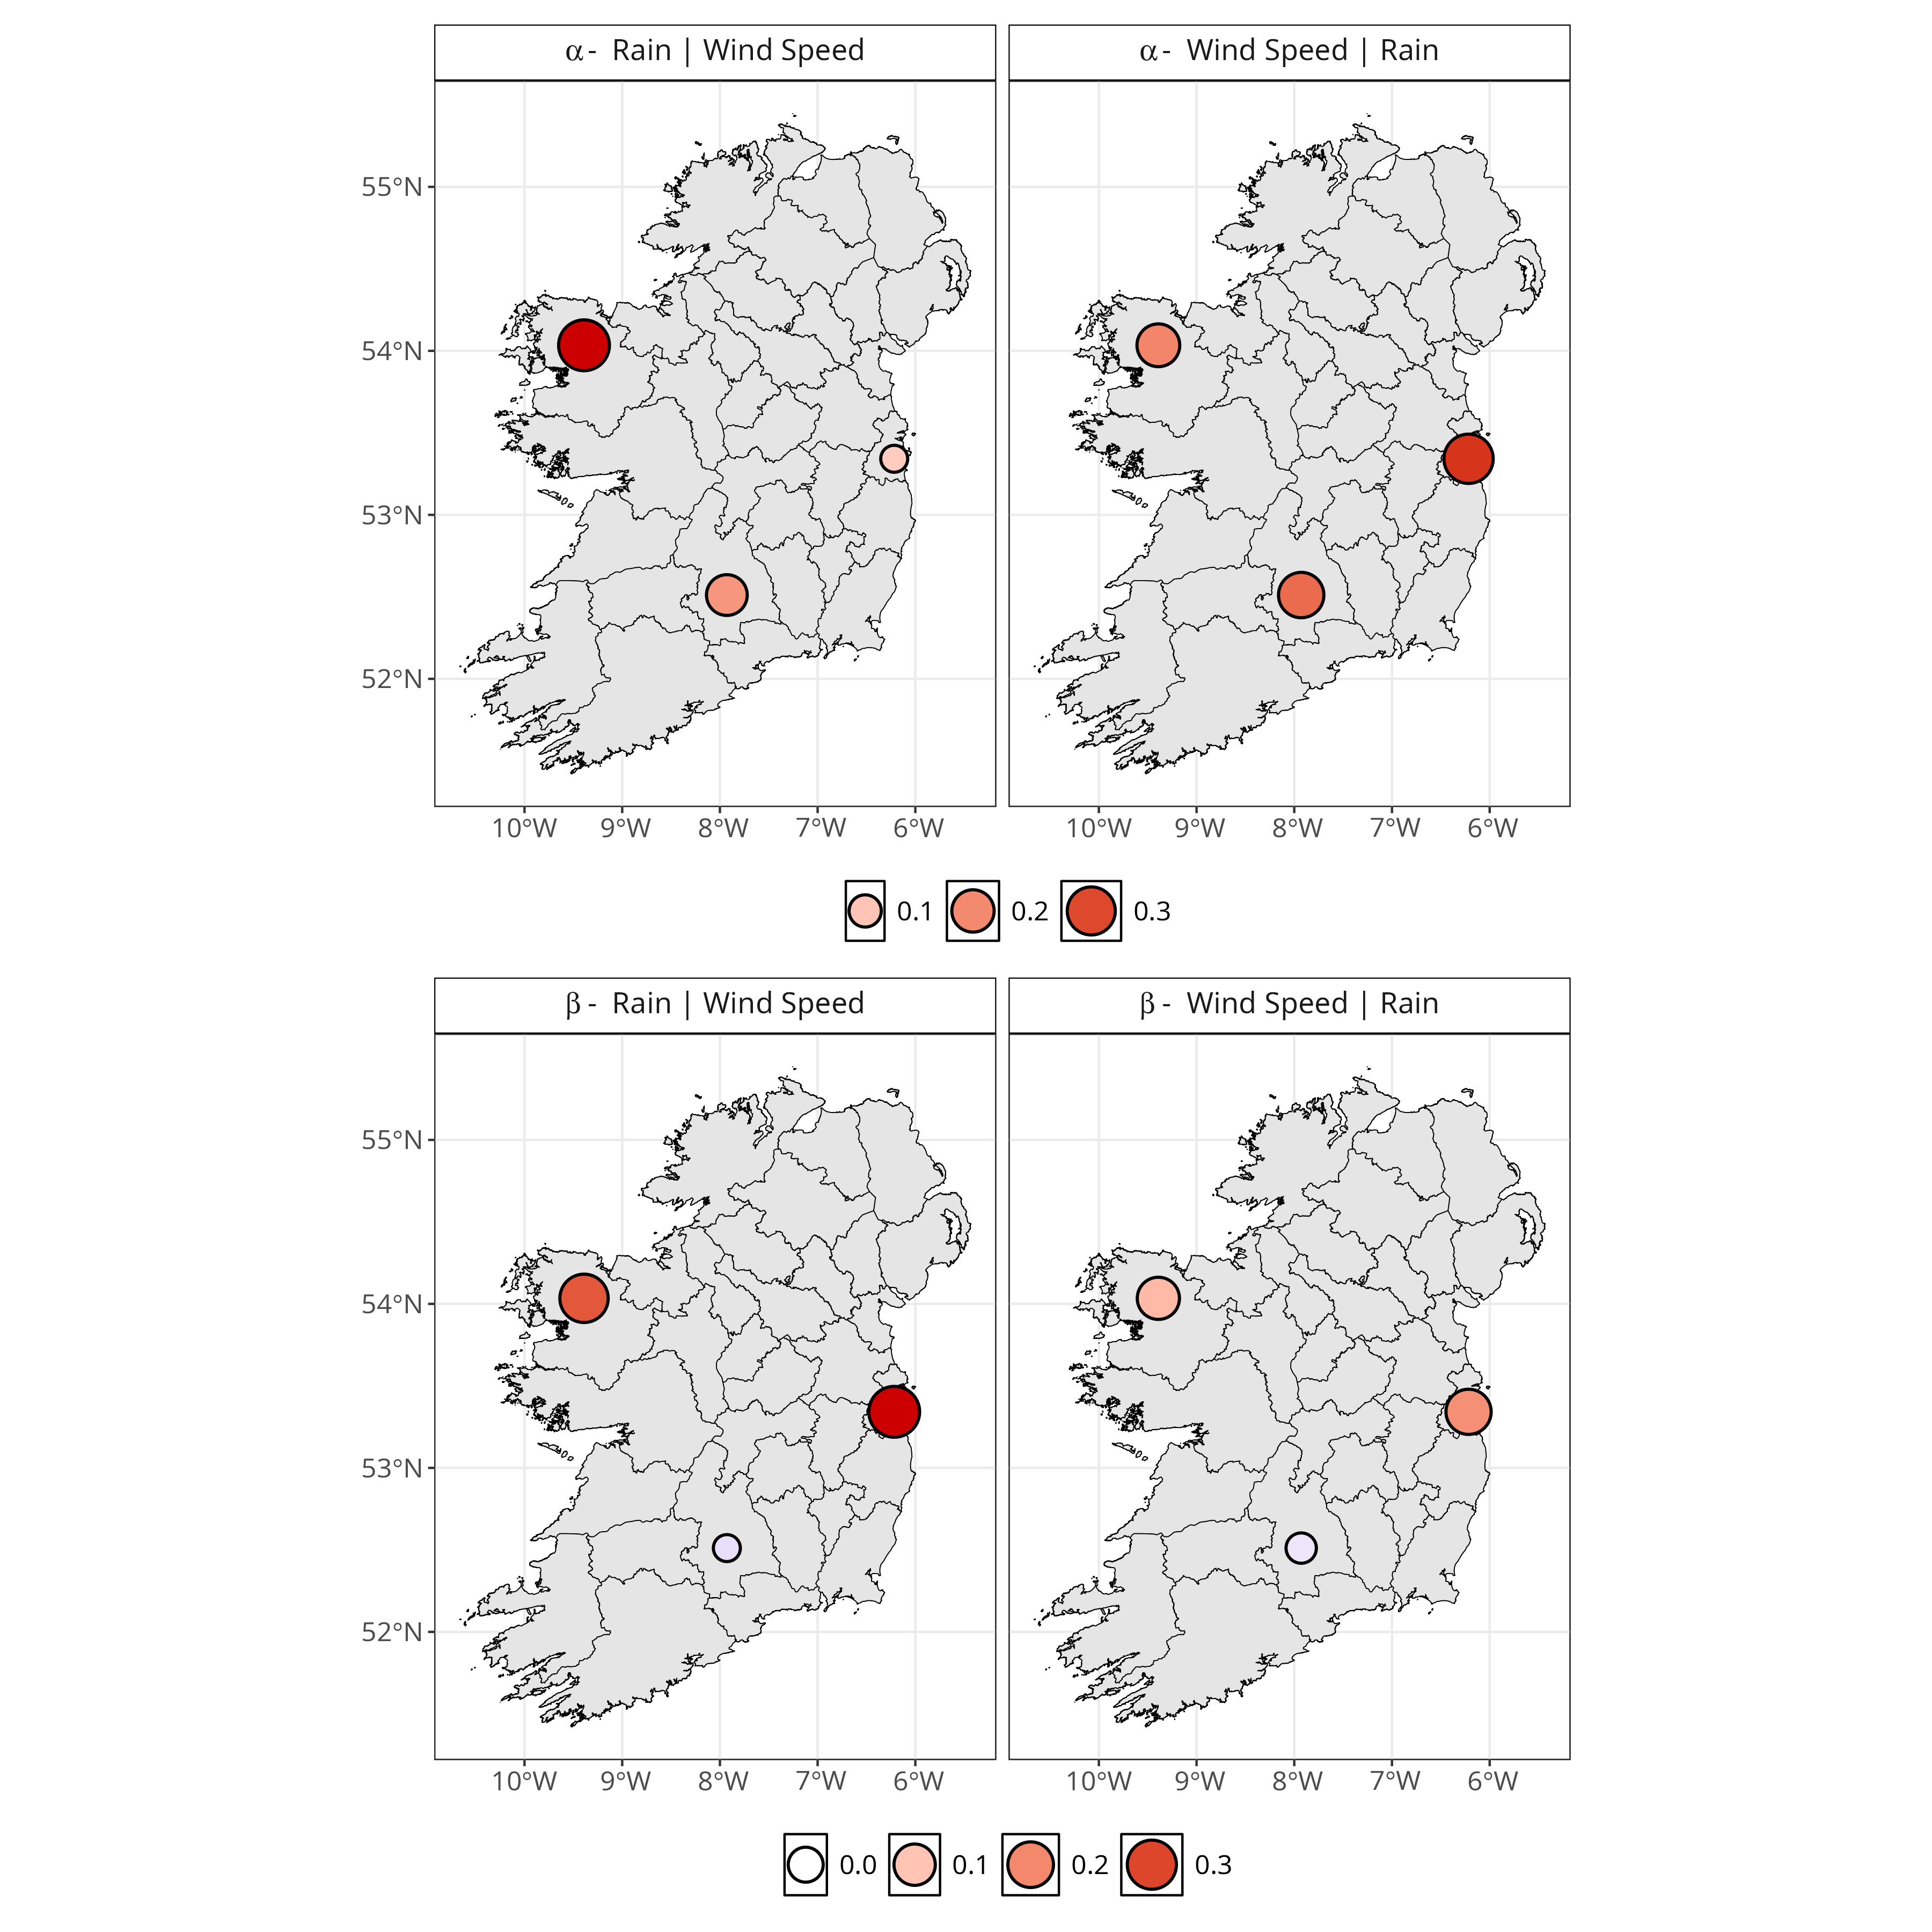
\includegraphics[width=0.72\textwidth]{plots/ab_map_post_clust.png}
\end{frame}

\end{document}
